%!TEX root = ../dissertation.tex

\chapter{Background and State of the Art}
\label{backgroundandsota}

In this chapter there will be an overview on essential concepts to understand this work, such as the representation of the eye orientation in the 3D space and the pinhole camera model. Some state of the art algorithms that can potentially solve the problem and enhance the solution will be presented. More specifically, the \acrlong{oppr}, optimization functions using the epipolar geometry relation and a robust estimation method are described.

%!TEX root = ../dissertation.tex
\section{Representation of eye orientation in 3 dimensions}
\label{cha2:represent}
In computer vision, it's customary to use the coordinate system on the left of Figure \ref{cha2:sec2:fig:coordsys2}, but in neuroscience a different convention, represented on the right of the Figure, is used. In order to be coherent with computer vision concepts, the first mentioned convention will be the one in use throughout the remaining of this report.

\begin{figure}[!htb]
	\centering
	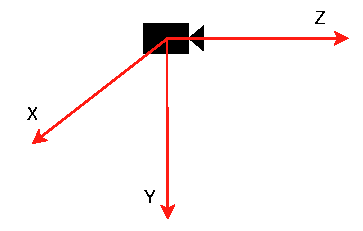
\includegraphics[width=0.41\textwidth]{images/cvcoordinatesys.pdf}
	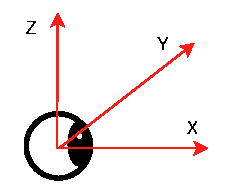
\includegraphics[width=0.25\textwidth]{images/cvcoordinatesysq.pdf}
	\caption[Computer Vision vs Neuroscience coordinate systems]{On the left, the coordinate system used in computer vision with the torsional component coming out of the front of the camera. On the right, the coordinate system used in the neuroscience field with the torsional component coming out of the front of the eye.}
	\label{cha2:sec2:fig:coordsys2}
\end{figure}

There are several ways of representing a rotation in 3D, the most common being Euler angles and rotation matrices. Euler angles are three angles that describe the orientation of a rigid body with respect to a fixed coordinate system. For this work, maintaining the coordinate system said above, the sequence of rotations used to represent a given orientation can be defined by the angles $[\theta_Z \ \theta_Y \ \theta_X]$, which corresponds to rotating around Z, Y, X axes, respectively.

\subsection{Rotation matrices}
\label{rotmatsss}
The human eye is a purely rotative body (no translations), and thus any orientation can be described by a unique series of three rotations around each of the axis defined in three dimensional space as
\begin{equation}
\label{rrr}
R _ { z } ( \theta_Z ) = \left[ \begin{array} { c c c } { \cos \theta_Z } & { - \sin \theta_Z } & { 0 } \\ { \sin \theta_Z } & { \cos \theta_Z } & { 0 } \\ { 0 } & { 0 } & { 1 } \end{array} \right], \
R _ { y } ( \theta_Y ) = \left[ \begin{array} { c c c } { \cos \theta_Y } & { 0 } & { \sin \theta_Y } \\ { 0 } & { 1 } & { 0 } \\ { - \sin \theta_Y } & { 0 } & { \cos \theta_Y } \end{array} \right], \
R _ { x } ( \theta_X ) = \left[ \begin{array} { c c c } { 1 } & { 0 } & { 0 } \\ { 0 } & { \cos \theta_X } & { - \sin \theta_X } \\ { 0 } & { \sin \theta_X } & { \cos \theta_X} \end{array} \right],
\end{equation}
where each angle is defined in counter-clockwise direction around each axis. An arbitrary rotation, $R$, may then be defined as some multiplication (i.e. a serial order) of those three, noting that the order by which they are multiplied matters (rotations are non-commutative). A matrix originated from any combination of those is a rotation matrix because it satisfies the following conditions,
\begin{align}
	\label{epwifneprnf}
	R^{-1} = R^T\\
	\label{ienvpirnf}
	det(R) = 1.
\end{align} 

Instead of using multiple rotations done after each other around three different axes, Euler's theorem states that the orientation of the rotating body can also be parametrized by a single rotation with an angle, $\rho$, about an axis in 3D, $\hat{\mathbf{n}} = (n_1, n_2, n_3)$. That rotation is denoted as $R(\hat{\mathbf{n}}, \rho)$ and is given by 
\begin{equation}
R ( \hat { \mathbf{n} } , \rho ) = \left( \begin{array} { c c c } { \cos \rho + n _ { 1 } ^ { 2 } ( 1 - \cos \rho ) } & { n _ { 1 } n _ { 2 } ( 1 - \cos \rho ) - n _ { 3 } \sin \rho } & { n _ { 1 } n _ { 3 } ( 1 - \cos \rho ) + n _ { 2 } \sin \rho } \\ { n _ { 1 } n _ { 2 } ( 1 - \cos \rho ) + n _ { 3 } \sin \rho } & { \cos \rho + n _ { 2 } ^ { 2 } ( 1 - \cos \rho ) } & { n _ { 2 } n _ { 3 } ( 1 - \cos \rho ) + n _ { 2 } \sin \rho } \\ { n _ { 1 } n _ { 3 } ( 1 - \cos \rho ) - n _ { 2 } \sin \rho } & { n _ { 2 } n _ { 3 } ( 1 - \cos \rho ) + n _ { 1 } \sin \rho } & { \cos \rho + n _ { 3 } ^ { 2 } ( 1 - \cos \rho ) } \end{array} \right).
\end{equation}

Still, rotation matrices are not the most efficient way to define rotations given they have nine elements and only three are actually necessary to describe the rotation uniquely. Hence, in oculomotor literature more suitable representations are used, such as quaternions, or rotation vectors that are more intuitive. \cite{rep}\cite{mathrot}

\subsection{Quaternions}
\label{cha2:represent:quat}
Quaternions are 4-dimensional complex algebraic objects that are related to a rotation around an axis, $\hat{ \mathbf{n}}$ by an angle $\rho$ as follows,
\begin{equation}
\label{sec2:eq:q}
q = \cos ( \rho / 2 ) + \mathbf{i} \sin ( \rho / 2 ) \mathbf{\hat{n}} \equiv q _ { 0 } + {\bf i}\cdot  {\bf q},
\end{equation}
where $q_0$ and $\mathbf{q} = [q_1 \ q_2 \ q_3]$ are the scalar and vectorial parts of the quaternion, respectively, and ${\bf i}$ is the complex 3D vector. 

Like rotation matrices, a quaternion can be defined as a sequence of rotations by multiplying each corresponding quaternion in sequence.
The product of a quaternion $\mathbf{q}$ with a quaternion $\mathbf{p}$ is 
\begin{equation}
	q_0 p_0 - \mathbf{q} \cdot \mathbf{p} + q_0 \mathbf{p} + p_0 \mathbf{q} + \mathbf{q} \times \mathbf{p}.
\end{equation}
The rotation between two quaternions can be obtained by 
\begin{equation}
\label{inrefiorenf}
\mathbf{p} \cdot \mathbf{q}^{-1},
\end{equation}
where $\mathbf{q}^{-1} = \frac{q^*}{|q|}$ with $q^*$ being the conjugate of $q$.

Moreover, quaternions can be related to rotation matrices through
\begin{equation}
	R=\left[\begin{array}{lll}{1-2\left(q_{2}^{2}+q_{3}^{2}\right)} & {2\left(q_{1} q_{2}-q_{0} q_{3}\right)} & {2\left(q_{1} q_{3}+q_{0} q_{2}\right)} \\ {2\left(q_{1} q_{2}+q_{0} q_{3}\right)} & {1-2\left(q_{1}^{2}+q_{3}^{2}\right)} & {2\left(q_{2} q_{3}-q_{0} q_{1}\right)} \\ {2\left(q_{1} q_{3}-q_{0} q_{2}\right)} & {2\left(q_{2} q_{3}+q_{0} q_{1}\right)} & {1-2\left(q_{1}^{2}+q_{2}^{2}\right)}\end{array}\right]
\end{equation}

For the description of eye movements, only the vectorial part, $\mathbf{q}$, is necessary, since the scalar part does not contain any information not already given by the vectorial one. Thus, it can be eliminated by using rotation vectors, which are related to quaternions  by $ \mathbf{r}  = {\bf q} / q _ { 0 }$.

\subsection{Rotation vector in head-fixed coordinates}
\label{killme}

The rotation vector, $\mathbf{r}$, is directed along the rotation axis, $\hat{\mathbf{n}}$, and its length varies with the amount of rotation, $\rho$, around it. It can be described by 
\begin{equation}
\mathbf{r} = \tan (\frac{\rho}{2}) \hat{ \mathbf{n}},
\end{equation}
where $\hat{ \mathbf{n}}$ can be obtained through a rotation matrix as
\begin{equation}
\label{sec2:eq:n}
\begin{aligned} 
n_ { 1 } & = \sin \rho \left( R _ { 32 } - R _ { 23 } \right) / 2  \\ 
n _ { 2 } & = \sin \rho \left( R _ { 13 } - R _ { 31 } \right) / 2  \\ 
n _ { 3 } & = \sin \rho \left( R _ { 21 } - R _ { 12 } \right) / 2 ,
\end{aligned}
\end{equation}
and $\rho$ through
\begin{equation}
\cos \rho = 1 / 2 \cdot \left( R _ { 11 } + R _ { 22 } + R _ { 33 } - 1 \right).
\end{equation}
It's important to note that in this format, the units are given in half-radians.

%!TEX root = ../dissertation.tex

\section{Camera Model}
\label{cha2:cameramodel}

In this section, are introduced the essential concepts on the pinhole camera model that follow. Digital cameras are equipped with a sensor (mostly charge-coupled devices, CCD, and CMOS') that transforms light into discrete electrical signals. When taking a picture, some of the light reflecting on the object is directed towards the camera pinhole (tiny aperture on the camera), forming a 180º inverted image of the object on the sensor, as shows on Figure \ref{cha2:sec2:fig:camera_concepts}. All the light rays entering the camera converge into the pinhole and diverge on the other side (with a unique one-to-one correspondence). Therefore the pinhole is also named the \textbf{center of projection}, principal point, or focal point.

In cameras the aperture size and light-exposure time can be controlled. A smaller aperture produces a sharper image but needs a longer exposure time to collect enough light, whereas a larger aperture allows more light to be captured, but at the expense of producing blurred images.

The image of the object is projected onto the so-called \textbf{image plane}. When moving this plane closer to the pinhole (zoom out), the projected object gets smaller, and vice-versa. The distance between the plane and the aperture is the \textbf{focal length}, or focal distance. The view-angle of a camera depends on the focal distance, and on the sensor size. The image resolution depends solely on the number of pixels that fit on the sensor.

A useful coordinate system, called the \textbf{camera reference system}, is centered at the pinhole, and has its z-axis perpendicular to the image plane, as mentioned in section \ref{cha2:represent}. The line defined between the center of projection and the center of the image plane is called the \textbf{optical axis}.

\begin{figure}[ht]
	\centering
	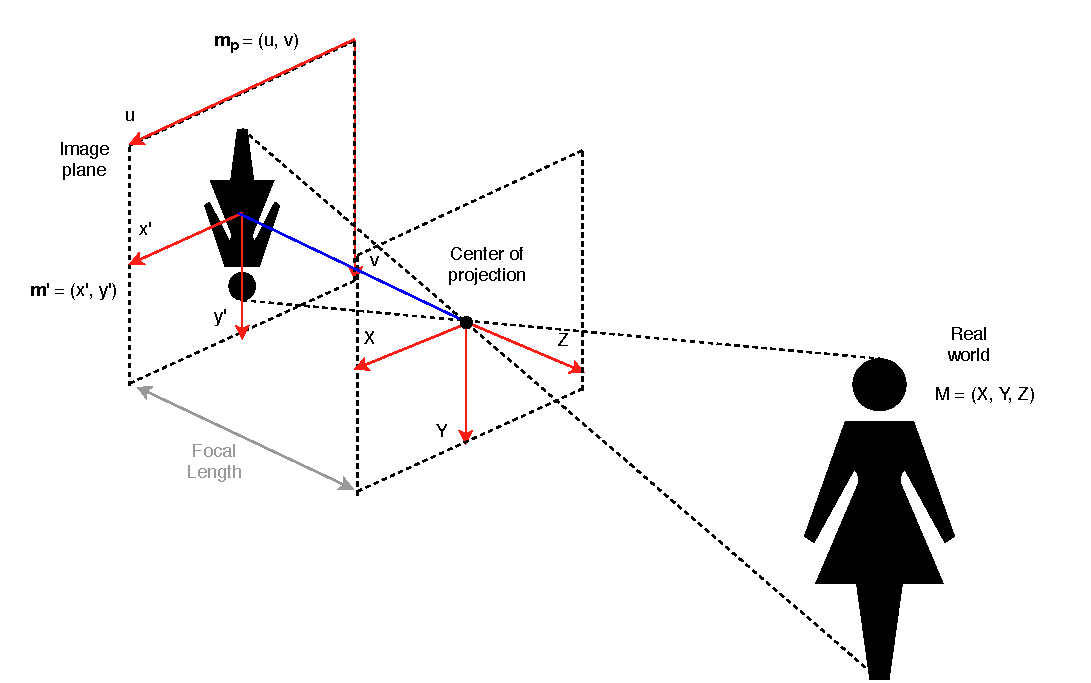
\includegraphics[width=\textwidth]{images/cameraconcepts.pdf}
	\caption[Pinhole Camera Model]{Pinhole Camera Model. The girl defined by the generic set of points $M$ is projected onto the image plane (defined by the set of generic points $\bf m_{p}$) through the light rays passing by the camera's pinhole, called the center of projection. The focal length is the distance from the center of the image plane to the center of projection. The digital image's coordinate system $(u, v)$ is defined on top right corner of the image plane. The optical axis is the blue line.}
	\label{cha2:sec2:fig:camera_concepts}
\end{figure}

Figure \ref{cha2:sec2:fig:camera_concepts} summarizes the concepts explained above, and helps at understanding the upcoming details. It's possible to establish a relationship between a real point in space and a point in an image in pixels, through the camera model as follows.

\begin{enumerate}
	\item \textbf{Passing from the world frame to the camera reference frame}
	
	An arbitrary real point in space $M_W = [X_W \ Y_W \ Z_W]^T$ may be represented in the world reference frame, so it needs to be be converted into the camera reference frame, becoming $M$.
	
	This conversion consists on expressing the origin of the world reference frame on the camera frame, through a translation, $\bf t$, and a rotation, that can be represented by a matrix, $R$. These are called the \textbf{extrinsic parameters}.
	\begin{equation}
		M = [X \ Y \ Z]^T = R \ [X_W \ Y_W \ Z_W]^T + \mathbf{t}
	\end{equation}
	
	\item \textbf{Project the 3D points into the image plane reference frame}
	
	As may be observed in the figure, a correspondence between the real world points $M = [X \ Y \ Z]^T$ and the points projected onto the image plane $\mathbf{m'} = [x' \ y']^T$ can be established by the following triangular similarity as
	\begin{equation}
	\label{cha2:sec2:eq:trisimilar}
	x' = f\frac{X}{Z}, \ y' = f\frac{Y}{Z},
	\end{equation}
	
	where $f$ is the focal length in meters, and $x', y', X ,Y$ and $Z$ are also represented in meters.	
	
	\item \textbf{Transform image plane points into pixel coordinates}
	
	The digital image obtained is actually expressed in pixel units, whereas till now everything was described in metric units, requiring the points to be converted by scalings $(s_x, s_y)$, as 
	\begin{equation}
	\label{cha2:sec2:eq:trisimilar}
	u_s = s_x x', \ v = s_y y',
	\end{equation}
	where $(u,v)$ are the scaled image coordinates in pixels, denoted by $\mathbf{m} = [u_s \ v_s]^T$.
	
	Moreover, the image plane center does not coincide with the center of the digital image reference frame, as shown in Figure \ref{cha2:sec2:fig:camera_concepts}, thus the image points also have to be translated by $(c_x \ c_y)$ pixels, which is camera's principal point offset. 
	\begin{equation}
	\label{cha2:sec2:eq:trisimilar}
	u_{sc} = s_x x' + c_x, \ v = s_y y' + c_y.
	\end{equation}
	
	Furthermore, due to sensor errors, there might be a deformation skew, $s$, associated to the camera reference frame, which means that it may not have exactly perpendicular axes.
	\begin{equation}
	\label{cha2:sec2:eq:trisimilar}
	u = s_x x' + sy' + c_x, \ v = s_y y' + c_y.
	\end{equation}
	Combining all the parameters, it yields the so-called \textbf{intrinsic parameters} matrix defined as,
	\begin{equation}
	\label{sec2:eq:kmatrix}
	K = \left[ 
	\begin{array} { c c c } 
	f s_x & s     & c_x \\ 
	0 	  & f s_y & c_y \\ 
	0     & 0     & 1   
	\end{array} 
	\right].
	\end{equation}
\end{enumerate}
Hence, using \gls{homo}, $\bf m$ may be expressed as,
\begin{equation}
\begin{array} { l } 
\mathbf{\widetilde{m}} = K R \frac{M}{Z} + \mathbf{t} \\
\lambda \mathbf{\widetilde{m}} = KR M +  \mathbf{t} 
\end{array},
\end{equation}
where $\lambda = Z$. Or, more commonly, 
\begin{equation}
\begin{array} { l } { \lambda \mathbf{\widetilde{m}} \sim K [ R \ | \ \mathbf{t} ] \widetilde { M } } \\ { \lambda \mathbf{\widetilde{ m }} \sim P \widetilde { M } } \end{array},
\end{equation}
where $P$ is a $3\times4$ matrix, named \textbf{camera matrix}.
	
In practice, the camera model contains several nonlinear effects, generically denoted as "distortion", since real cameras have lenses instead of a pinhole. The lens allows all the emitted rays of light to be refracted into one converging point, the focal point. Although the focal length will now increase the distance from the lens to the converging point, the camera model explained above still applies, but the distortions must be accounted for. These distortions are incorporated in (\ref{cha2:sec2:eq:radiald}). Radial distortion is modeled by the $k_i$ coefficients on the left-hand side of the polynomial transformation in (\ref{cha2:sec2:eq:radiald}) (taken from Zernike's model of aberrations), and the tangential distortion (which occurs when the image plane is not parallel to the camera lens) is defined by the $p_j$ coefficients in the right-hand term.\footnote{Born, Max; Wolf, Emil. Principles of Optics: Electromagnetic Theory of Propagation, Interference and Diffraction of Light. Chapter 5.} 

\begin{equation}
\label{cha2:sec2:eq:radiald}
\begin{array} { l } 
{ x' _d = x' \ \frac{ 1 + k_1 r^2 + k_2 r^4 + k_3 r^6}{ 1 + k_4 r^2 + k_5 r^4 + k_6 r^6}  +  ( 2 p_1 x' y' + p_2 ( r^2 + 2 x'^2) )}\\ 
{ y' _d = y' \ \frac{ 1 + k_1 r^2 + k_2 r^4 + k_3 r^6}{ 1 + k_4 r^2 + k_5 r^4 + k_6 r^6} +  ( p_1 ( r^2 + 2 y'^2 ) + 2 p_2 x' y')}
\end{array},
\end{equation}
where $r^{2} = {x'}^{2} + {y'}^{2}$ and ${x'}_d$ and ${y'}_d$ are the distorted coordinates of the image point, which should then be converted into digital image coordinates as shown previously. 

%!TEX root = ../dissertation.tex

\section{Feature detection and matching}
\label{cha2:features}

As explained before on section \ref{cha1:problemdef}, it is necessary to gather corresponding features in consecutive images taken before and after a rotation, and to use an algorithm to estimate the orientation using those features. The latter, also referred to as keypoints or interest points, are spatial locations of an image that "stand out", allowing it to be identifiable. This points should be such that even after rotating, translating, shrinking or distorting the image, they can be found.

It is absolutely necessary to have a solid detection and trust-worthy correspondence of image features (matching) when doing an "eye" movement to eventually estimate the its current orientation.

Two main approaches exist to the problem of feature detection and matching. The first method finds features in one image and matches these features in the other image. The second method, which is more suitable for points in the near space, independently detects features in both images and subsequently matches them on the basis of local correspondences.

It might not be appropriate to extract features from an image having high detail (i.e. high spatial bandwidth) on the finest stable scale possible, because when matching features with another image at a different (coarser) scale those details may no longer be detectable. Therefore, it's important to extract features at a variety of scales to ensure their invariance. 

Besides scale, preserving rotation and orientation invariance is also a concern. One way to deal with this problem is to define a descriptor. This is a scaled and oriented patch around the chosen point with the local orientation and scale, from which the dominant orientation can be extracted to guarantee its invariance. \cite{multiview}

There exist a number of algorithms that can do the job. However, none of these algorithms is optimal for all images, as each of them is optimized for particular computer vision applications, with performance depending heavily on the environmental properties (illumination, image quality, contrast, ...). A comprehensive survey on the state of the art of feature detection and description  \cite{featsift} (by Salahat E. and Qasaimeh M. in 2017), proposes that ideal features should have the following properties:
\begin{itemize}
	\item Distinctiveness: the gradient variations surrounding the point should be sufficiently large;
	\item Locality: to avoid obstruction and deformation between the two images.
	\item Quantity: enough features to describe the content;
	\item Accuracy: features should be accurate enough to be detected independently of image scale, shape or pixel location;
	\item Efficiency: be detected fast enough for real-time systems;
	\item Repeatability: a high percentage of features should be detected in both images on the overlapping regions;
	\item Invariance: deformative effects on the features, due to scaling, rotation or translation are minimized;
	\item Robustness: features should be less sensitive to deformations due to noise, blur, compression, and so on.
\end{itemize} 
The review paper also presents an overview on the recent algorithms proposed on this matter, comparing them in terms of the metrics defined above. The analysis in that article suggests that MSER (Maximally stable extremal regions) and SIFT (\acrlong{sift}) algorithms enhance performance on computational complexity, accuracy and execution time. From the scale and rotation invariant algorithms, SURF (\acrlong{surf}), proved to be faster than \acrshort{sift}, although not as robust.

MSER (by Matas J. in 2002)\footnote{J. Matas J., O. Chum, M. Urban and T. Pajdla, “Robust Wide Baseline Stereo from Maximally Stable Extremal Regions,” 2002.} are areas of uniform intensity outlined by contrasting backgrounds. They are constructed by trying multiple thresholds on the input image. The ones that remain unchanged in shape over the range of thresholds are the potential features to be selected as areas of interest. The centroids of these areas can subsequently be used to create a feature descriptor for the matching step.

\acrshort{sift} (by Lowe, David G. in 2004) \cite{sift} algorithm detects image features using a Gaussian filter by generating increasingly blurred images, and subtracting each image to each other. This is done in several scales in order to provide scale invariance. Afterwards, a descriptor for each feature at a certain scale is created and includes information about the orientation and gradient magnitude around the point, which also grants rotation invariance.

\acrshort{surf} (by Bay, Herbert in 1999) \cite{surf} uses an integral image, which is an intermediate representation of the original image where the value of a location is the sum of all pixels of a rectangular region formed around that location. This is called box filter and serves as an approximation to the \gls{gauss}, speeding up the process in relation to \acrshort{sift}.

A more comprehensive explanation on both SIFT and SURF can be found at appendix \ref{appendix:cha1:sec1:sift} and \ref{appendix:cha1:sec1:surf}, respectively. Any of these 3 algorithms mentioned seems promising to use as feature detector in this work.

\subsection{Matching step}
Regarding the matching of feature descriptors, one of the most common search algorithms used is the Nearest Neighbor Search. FLANN (\acrlong{flann}) (by M. Muja in 2009) \footnote{M. Muja and D. Lowe, “Fast approximate nearest neighbors with automatic algorithm configuration,”, 2009.} provides a library for performing this kind of searches in high-dimensional spaces. It contains a collection of algorithms that the authors found to  work best for nearest neighbor search and a system for automatically choosing the best algorithm and optimum parameters depending on the dataset.


%!TEX root = ../dissertation.tex

\section{Orthogonal Procrustes Problem and Lack of Depth}
\label{cha2:opprandsphere}

Assuming that the image points are obtained from the RGB camera installed on the eye prototype, using the camera model, this 2D points can be converted to corresponding points in space. 

The 3D points can then be used to estimate the rotation executed by the eye. There are several ways to do this, a potential one is \acrfull{oppr}. This algorithm finds the optimal linear transformation between two 3D clouds of points.

Procrustes, the son of Poseidon in Greek mythology, made his victims fit in a wonderful all-fitting bed, either by stretching their limbs, or by cutting them off. Ultimately, he was fitted into his own bed by Theseus.\footnote{Karl Kerenyi, The Heroes of the Greeks, 1959:223, noting pseudo-ApollodorusDiodorus Siculus, 4.59.5.} This is similar to the analysis held here, there are 3 elements to Procrustes's problem: $M_2$, the bed, $M_1$, the unlucky adventurer, and T, the fitting treatment. The solution to the problem is a matrix, T, that minimizes
\begin{equation}
\label{sec2:eq:procrustes}
\left \| M_2 - TM_1  \right \|^2 ,
\end{equation}
which transforms $M_1$ into $M_2$. $M_1$ and $M_2$ are clouds of 3D points obtained from the images took from the perspectives before and after a rotation, defined as $R$. Hence, the function to minimize is
\begin{equation}
\label{sec2:eq:ptrace}
\left \| M_2 - RM_1 \right \|^2 
\end{equation}
that through the Frobenius norm can be expanded as
\begin{equation}
\label{sec2:eq:ptrace}
\left \| M_2 - RM_1 \right \|^2 = \operatorname { trace } ( M_2^T M_2 + M_1^T M_1) - 2 \operatorname { trace } (M_2^T R M_1).
\end{equation}
This means that minimizing (\ref{sec2:eq:procrustes}) with respect to $R$ is equivalent to maximizing the second term of (\ref{sec2:eq:ptrace}). By applying \gls{svd} (SVD) to $M_1 M_2^T$, the latter term can be further simplified into
\begin{equation}
\label{sec2:eq:svd}
\operatorname { trace } (M_2^T R M_1) = \operatorname { trace } (M_1 M_2^T  R) = \operatorname { trace } ( U \Sigma V^T R) = \operatorname { trace } (\Sigma V^T R U) = \operatorname { trace } (\Sigma H )  = \sum _ { i = 1 } ^ { N } \sigma _ { i }h _ { i i } .
\end{equation}
The singular values of $\sigma _ { i }$ are all non-negative, and so the expression becomes maximum when $h _ { i i } = 1$ for $i=1,2,...,N$, since $H$, a product of orthogonal matrices, is an orthogonal matrix itself, thus having its maximal value when $H = I$. This results in $I = V^T R U$, obtaining $R=V U^T$ as the rotation of the eye.   

When $M_1$ and $M_2$ are associated with different origins, it is customary to consider  better fits of the configurations by allowing shape-preserving translations of the origin.
When translating the points clouds by $t_1$ and $t_2$, respectively, (\ref{sec2:eq:procrustes}) becomes
\begin{equation}
\label{sec2:eq:strans1}
\left \|(M_2 - \mathbf{1} \mathbf{t_2}^T) - R(M_1 - \mathbf{1} \mathbf{t_1}^T)\right \|^2,
\end{equation}
which can also be written as
\begin{equation}
\label{sec2:eq:strans2}
\left \| M_2  - RM_1 - \mathbf{1} \mathbf{t}^T\right \|^2,
\end{equation}
where $\mathbf{t}^T = \mathbf{t_2}^T - R\mathbf{t_1}^T$. The expression is minimized when $\mathbf{t}^T$ corresponds to the column-means of $M_2 - RM_1$, therefore a simple way of effecting this translation is to remove the column-means of $M_1$ and $M_2$, separately, before minimizing, which is called centering. The data then becomes expressed in terms of the mean deviations. \cite{procrustes} 

However, in order to obtain the 3D point clouds from the \acrshort{rgb} images, taken before and after rotation, it is necessary to have the depth $\lambda$ that corresponds to the $Z$ coordinate in the real world, as seen on section \ref{cha2:cameramodel}. Assuming pure rotation, any depth provides the same information, so it's possible to define an artificial depth by projecting the 2D points in a sphere with enough radius compared to the focal length, as follows
\begin{equation}
	\label{cha2:sec3:eq:spherepro}
	\left \| (\lambda \mathbf{m_1'})  \right \| = \left \| (\lambda x_1', \lambda y_1', \lambda)  \right \| = r
\end{equation}
where $r$ is the radius of the sphere and $\lambda$ then becomes
\begin{equation}
	\label{cha2:sec3:eq:lamdba}
	\lambda = \frac{r}{\sqrt{x'^2 + y'^2 + 1}},.
\end{equation}
Yet, this makes centering inapplicable. Thus to use this algorithm, the translation associated to the eye movement in the current eye prototype has to be ignored, making the rotation derived from \acrshort{oppr} a mere approximate estimation.

%!TEX root = ../dissertation.tex

\section{Epipolar Geometry}
\label{cha2:epipolar}

Epipolar geometry provides an alternative yet powerful tool to obtain image transformations using various different approaches. It describes the relation between two images, before and after a transformation, through a 3x3 singular, non-invertible, matrix called the \textbf{essential matrix}, \textbf{$E$}, if the camera matrix is known, or the \textbf{fundamental matrix}, \textbf{$F$}, otherwise. These matrices are singular because they express an under-constrained relationship between a point in one image and its possible location in the other image, which is not unique due to depth ambiguity. The essential matrix is the product of a rotation matrix and a \gls{skews}, whose determinant is zero, as it will be shown below. If a point in the real world, $M$, is projected as a point $\mathbf{{m}_1}$ in the first image, and point $\mathbf{{m}_2}$ in the second, then those points satisfy the epipolar relation
\begin{equation}
\label{sec2:eq:epipolar}
\mathbf{\tilde{m}_2}^T F \mathbf{\tilde{m}_1} = 0,
\end{equation}
\begin{figure}[h]
	\centering
	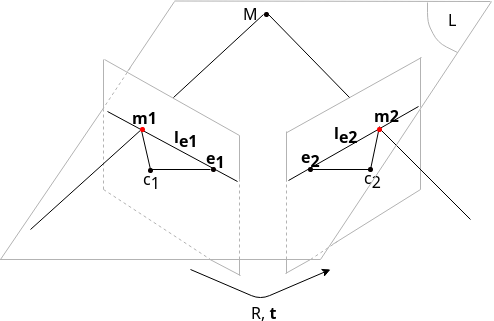
\includegraphics[width=11cm]{images/epipolargeo.png}
	\caption[Epipolar geometry]{Epipolar geometry. The two small vertical planes correspond to the image planes after the rotation and translation of the camera, $R$ and $\bf t$, respectively. $c_1$ and $c_2$ are the centers of projection before and after the transformation. $M$ is the fixed point gazed at in the real world. $\bf m_1$ and $\bf m_2$ are the projections of point $M$ into the respective image planes, whose rays are lying on the plane $L$. $\bf l_{e1}$ and $\bf l_{e2}$ are the epipolar lines, that also lie on the plane and $\bf e_1$ and $\bf e_2$ are the epipoles.}
	\label{sec2:fig:epipolargeo}
\end{figure}
which can be easily deduced with projective geometry. In Figure \ref{sec2:fig:epipolargeo}, $c_1$ and $c_2$ are the centers of projection before and after the camera has been displaced by $(R, \mathbf{t})$. Given the point $\bf m_1$ on the first image, its correspondence, $\bf m_2$, in the second image is constrained to a line, the epipolar line, $\bf l_{e2}$. The latter is defined as the intersection of the plane $L$ and the second image plane. Furthermore, plane $L$ is delineated by the two centers of projection and $\bf m_1$. The epipoles, $\bf e_1$ and $\bf e_2$, are born from the intersection of the line $c_1 - c_2$ with the epipolar lines, $\bf l_{e1}$ and $\bf l_{e2}$. 

\subsection{Projective geometry concepts}

To understand the upcoming deductions, let's introduce the following concepts.
\subsubsection{Representation of lines in \gls{homo}}
A line in a plane is represented by $a x + b y + c = 0$, which can also be defined by a vector $( a , b , c ) ^T$. For any non-zero constant, $k$, the vectors  $( a , b , c ) ^T$ and $k(a , b , c ) ^T$ represent the same line and are equivalent. An equivalence class of vectors is known as an homogenous vector. 
\subsubsection{Point lying on a line}
A point $\mathbf { p } = ( p_1 , p_2 ) ^ T$ lies on a line $\mathbf {\tilde{l}} = ( a , b , c ) ^ { T }$, if and only if $a p_1 + b p_2 + c = 0$, which can be written as $( p_1 , p_2 , 1 ) ( a , b , c ) ^T = \mathbf { \tilde{p} } ^T \mathbf {\tilde{l}} = \mathbf {\tilde{l}} ^T \mathbf { \tilde{p} } = 0$.
\subsubsection{Line joining points}
A line passing through any two points $\mathbf{\tilde{p}}$ and $\mathbf{\tilde{q}}$ can be defined by the cross-product of those points as $\mathbf{\tilde{l}} = \mathbf{\tilde{p}} \times \mathbf{\tilde{q}}$.
\subsubsection{Cross product's \gls{skews} representation}
The previous cross product, $\mathbf{\tilde{l}} = \mathbf{\tilde{p}} \times \mathbf{\tilde{q}}$, can be written as $\mathbf{\tilde{l}} = [\mathbf{\tilde{p}}]_{\times} \mathbf{\tilde{q}}$, where $[\mathbf{p}]_{\times}$ is a skew symmetric matrix defined as
\begin{equation}
\left[ \begin{array} { c c c } { 0 } & { - p_ { 3 } } & { p_{ 2 } } \\ { p_{ 3 } } & { 0 } & { - p_{ 1 } } \\ { - p _ { 2 } } & { p_ { 1 } } & { 0 } \end{array} \right]
\end{equation}.

\subsection{Deducing the fundamental matrix algebraically}

The derivation of the fundamental matrix uses the following facts,
\begin{enumerate}
	\item there is an \gls{homography} mapping via $L$ plane from the points of the first to the second image, characterized by $\mathbf{\tilde{m}_2} = H_M \mathbf{\tilde{m}_1}$;
	\item because $\mathbf{m_2}$ lies on $\mathbf{\tilde{l}_{e_2}}$, then $\mathbf{ \tilde{m}_2 } ^T \mathbf{\tilde{l}_{e_2}} = 0$;
	\item and since $\mathbf { e_2 }, \mathbf { m_2 } \in \mathbf{\tilde{l}_{e_2}}$, then $\mathbf{\tilde{l}_{e_2}} = [\mathbf{\tilde{e}_2}]_{\times} \mathbf{\tilde{m}_2}$.
\end{enumerate}
From 1) and 3), 
\begin{equation}
\label{ggg}
\mathbf{\tilde{l}_{e_2}} = [\mathbf{\tilde{e}_2}]_{\times} H_M \mathbf{\tilde{m}_1} 
\end{equation}
can be deduced and using conclusion 2) and (\ref{ggg}),
\begin{equation}
\label{sec2:eq:fundm}
\mathbf{\tilde{m}_2}^T \mathbf{\tilde{l}_{e_2}} = 0 = \mathbf{\tilde{m}_2}^T [\mathbf{\tilde{e}_2}]_{\times} H_M \mathbf{\tilde{m}_1}  = \mathbf{\tilde{m}_2}^T F \mathbf{\tilde{m}_1},
\end{equation}
where $F$, the fundamental matrix, is an homogeneous matrix of rank-2 (since $[\mathbf{\tilde{e}_2}]_{\times}$ is rank-2 and $H_M$ is rank-3) with 7 degrees of freedom, and $det(F) = 0$.

\subsection{Deducing the fundamental matrix from camera motion}
Another way of obtaining this relation is through the camera motion.
If the point in the real world is expressed in the eye's perspective before rotating, $M_1$, under the camera model studied in section \ref{cha2:features}, (\ref{sec2:eq:eproj1}) and ((\ref{sec2:eq:eproj2}) are true and (\ref{sec2:eq:eproj3}) can be derived from them.
\begin{align}
\label{sec2:eq:eproj1}
\lambda_1 \mathbf{\tilde{m}_1} = K \tilde{M_1}, \\
\label{sec2:eq:eproj2}
\lambda_2 \mathbf{\tilde{m}_2} = K [ R \ \mathbf{t} ] \tilde{M_1}\\
\label{sec2:eq:eproj3}
\lambda_2 \mathbf{\tilde{m}_2} = K [ R \ \mathbf{t} ] K^{-1} \lambda_1 \mathbf{\tilde{m}_1}
\end{align}
For the sake of simplicity, the intrinsics matrix will be considered the identity, $K= I$, and the scale factors $\lambda_1$ and $\lambda_2$ will be dropped. Hence, by eliminating $\tilde{M_1}$, the previous equations become
\begin{equation}
\label{sec2:eq:elimp}
\mathbf{\tilde{m}_2} = R   \mathbf{\tilde{m}_1} + \mathbf{t},
\end{equation}
and because the cross product of two vectors is orthogonal to them both,  
\begin{align}
	\label{sec2:eq:fundm1}
	\mathbf{\tilde{m}_2}^T \cdot ( \mathbf{\tilde{m}_2} \times \mathbf{t}) = 0 \\
	\label{sec2:eq:fundm2}
	\text{and } ( \mathbf{\tilde{m}_2}^T\cdot((R  \mathbf{\tilde{m}_1} + \mathbf{t}) \times \mathbf{t}) = 0.
\end{align}
Therefore, the fundamental matrix, $F$, can be determined by 
\begin{equation}
\label{sec2:eq:fundm3}
\begin{aligned}
\mathbf{\tilde{m_2}}^T [\mathbf{t}]_\times R \mathbf{\tilde{m_1}} = 0 \\
\mathbf{\tilde{m_2}}^T F \mathbf{\tilde{m_1}} = 0.
\end{aligned}
\end{equation}
When the intrinsic parameters are not the identity matrix, then 
\begin{equation}
\begin{aligned}
\label{hhh}
\mathbf{\tilde{m_2}}^T K^{-T} E K^{-1} \mathbf{\tilde{m_1}} = 0 \\
\text{and finally }
F = K^{-T}  E K^{-1},
\end{aligned}
\end{equation}
where $E$ is the essential matrix.

\subsection{Estimating the fundamental matrix}
\label{einvonrev}
Having seen how the fundamental matrix is obtained from the known rotation and translation of a camera, the question now is how to determine $F$, and consequently the rotation, given two images with matching points. With the points referred to as $\mathbf{m_{1}} = [u_{1} \ v_{1}]^T$ and $\mathbf{m_{2}} = [u_{2}  \ v_{2}]^T$, the epipolar equation (\ref{sec2:eq:epipolar}) can then be written as
\begin{equation}
\begin{aligned}
\begin{bmatrix}
u_2 & v_2 & 1
\end{bmatrix}
\begin{bmatrix}
f_{11} & f_{12} & f_{13}  \\
f_{21} & f_{22} & f_{23}  \\
f_{31} & f_{32} & f_{33} 
\end{bmatrix}
\begin{bmatrix}
u_{1} \\ v_{1} \\ 1
\end{bmatrix}\\
=
\begin{bmatrix}
f_{11} u_1 u_2 + f_{12} v_1 u_2  + f_{13}u_2 + f_{21} u_1 v_2  + f_{22} v_1 v_2  + f_{23}v_2  + f_{31} u_1 + f_{32} v_1 + f_{33} 
\end{bmatrix}\\
=
\begin{bmatrix}
u_1u_2 \ v_1u_2 \ u_2 \ u_1v_2 \ v_1v_2 \  v_2 \ u_1 \ v_1 \ 1 
\end{bmatrix}
\begin{bmatrix}
f_{11} \ f_{12} \ f_{13} \ f_{21} \ f_{22} \ f_{23} \ f_{31} \ f_{32} \ f_{33}
\end{bmatrix}^T\\
= \mathbf{u} \cdot \mathbf{f}\\ = 0
\end{aligned}
\end{equation}
For $n$ pairs of points the expression becomes 
\begin{equation}
\label{sec2:eq:nsets}
U f = 0,
\end{equation}
where $U = \left[ \mathbf{u_ { 1 }} , \cdots , \mathbf{u_ { n }} \right] ^ { T }$. 
This linear homogeneous equation, and the rank-2 constraint over $F$, that restrains the matrix to 7 degrees of freedom (since $F$ is also defined up a scalar factor), will permit its unique identification. 
Hence, the estimation of $F$ may be done using only 7 point matches, or by using 8 or more if enough data points are available. In the latter case, the solution produced is in general unique, and there are several techniques to obtain it. In Zhang 1996's review on the issue \cite{detep}, the conclusion was that linear techniques are usually sensitive to noise and not very stable, because they ignore the constraints of $F$ and the minimization criterion is not physically meaningful. However, the results could be improved by using normalized data points instead of pixel coordinates. 

Nevertheless, non-linear optimization techniques seem to yield better results to the estimation problem of $F$. Three nonlinear algorithms are mentioned in the review paper \cite{detep} and in R. Hartley and A. Zisserman \cite{multiview}: (i) a minimization of the re-projection errors, (ii) a minimization of the symmetric epipolar error, (iii) and a minimization of the first order geometric error. The first one is the most time-consuming, thus not recommended. From the other two most promising approaches, the second seems to give the worst results and the last algorithm has been proposed to give the best results in the least amount of computational time. 

Algorithm (i), also called the Gold Standard, estimates $F$ by minimizing the distances between the points in the image and its re-projections. Having $M_1$ as a point in space, the corresponding points in the images before and after rotating are $\widetilde{\mathbf{m}}_{1}$ and $\widetilde{\mathbf{m}}_{2}$, respectively, obtained through  (\ref{sec2:eq:eproj1}) and ((\ref{sec2:eq:eproj2}).
The re-projections of $\widetilde{\mathbf{m}}_{1}$ and $\widetilde{\mathbf{m}}_{2}$ are then, 
\begin{align}
\label{cha2:epipolar:shitshit1}
	\lambda_2 \mathbf{\tilde{m}^r_2} = K [ R \ \mathbf{t} ] K^{-1} \lambda_1 \mathbf{\tilde{m}_1}\\
\label{cha2:epipolar:shitshit2}
	\lambda_1 \mathbf{\tilde{m}^r_1} =  K [ R^{T} \ -R^{T}\mathbf{t} ] K^{-1}  \lambda_2 \mathbf{\tilde{m}_2},
\end{align}
where $R$ and $\mathbf{t}$ are obtained from the factorization of $F$, that will be approached briefly on section \ref{cha2:epipolar:fact}, $K$ are the known intrinsic parameters of the camera and $\lambda_1$ and $\lambda_2$ are given by the projection of the points on a sphere mentioned on section \ref{cha2:opprandsphere}. The distance between $\widetilde{\mathbf{m}}_{1}$ and $\widetilde{\mathbf{m}}^r_{1}$ is defined by $|| \widetilde{\mathbf{m}}_{1} - \widetilde{\mathbf{m}}^r_{1} ||$, leading to the following cost function to minimize 
\begin{equation}
\label{cha2:sec3:eq:gold}
	\min_{\mathbf{F}} \sum_{i}
	||\widetilde{\mathbf{m}}_{1i} - \widetilde{\mathbf{m}}^r_{1i}||^2
	+
	||\widetilde{\mathbf{m}}_{2i} - \widetilde{\mathbf{m}}^r_{2i}||^2,
\end{equation}
where $i=1,...,n$.

Algorithm (ii) minimizes the epipolar error symmetrically, which is the distance from a point to its epipolar line. Having the epipolar line of the first image as $\widetilde{\mathbf{l}}_{e_1} =  F\widetilde{\mathbf{m}}_{2}$ and the second's as $\widetilde{\mathbf{l}}_{e_2} =  F\widetilde{\mathbf{m}}_{1}$, as shown on \ref{sec2:eq:fundm}, the quantity to minimize is given by
\begin{equation}
	\min _{\mathbf{F}} \sum_{i}\left(d^{2}\left(\mathbf{m}_{2i}, \mathbf{l}_{e_{2}}\right)+d^{2}\left(\mathbf{m}_{1i}, \mathbf{l}_{e_{1}}\right)\right),
\end{equation}
where $d\left(\mathbf{p}, \mathbf{l}\right)=\frac{a p_{1}+b _{2}+c}{\sqrt{a^{2}+b^{2}}}$, with $\widetilde{\mathbf{l}} = (a, b, c)^{T}$
and $\mathbf{p}=\left(p_{1}, p_{2}\right)^{T}$, is the distance of a point to a line.

Minimizing $ \sum_i (\mathbf{\widetilde{m_i}}'^T F \mathbf{\widetilde{m_i}})^2$ doesn't yield a good result because the variance of each $i$ term is not the same and the least-squares technique produces an optimal solution if each term has the same variance. So one possibility is to determine the fundamental matrix the way it's given by algorithm (iii), 
\begin{equation}
\min_F \sum_i \frac{ (\mathbf{\widetilde{\mathbf{m}}_{2i}}^T F \widetilde{\mathbf{m}}_{1i})^2}{\sigma_i^2},
\end{equation}
where $\sigma_i^2$ is the variance given by 
\begin{equation}
\sigma_i^2 = \sigma [l_{{e1i}_x}^2 + l_{{e1i}_y}^2 + l_{{e2i}_x}^2 + l_{{e2i}_y}^2].
\end{equation}
This corresponds to minimizing the derivative of the epipolar relation, thus its also called \acrfull{grat}, or the Sampson error.
Because multiplying each term by a constant makes no difference, $\sigma$ can be dropped. 

\subsection{Factorization of the essential matrix}
\label{cha2:epipolar:fact}
Once the fundamental matrix is obtained through one of those methods, assuming the intrinsic parameters are known, which is the case for this work, the essential matrix may be obtained by $E = K^{T}  F K$ as seen on (\ref{hhh}).
From here, it's possible to retrieve the camera matrix, $P = [R \ | \ \mathbf{t}]$, since $E = [\mathbf{t}]_\times R$, so that the rotation, $R$, and thus the orientation of the camera becomes known.
To find the camera matrix, one can apply the \acrshort{svdd} to the essential matrix, which generates 4 possible solutions,
\begin{equation}
P = \left[UWV^T | + u_{ 3 } \right] \quad \text { or } \quad \left[ UWV^T | - u_ { 3 } \right] \quad \text { or } \quad \left[ UW^T V^T | + u_ { 3 } \right] \quad \text { or } \quad \left[ UW^T V^T |- u _ { 3 } \right],
\end{equation}
that are represented by (a), (b), (c) and (d), respectively, on Figure \ref{sec2:fig:ep4} \footnote{The way this solutions are obtained is further detailed on appendix \ref{appendix:cha1:epipolar}.}. $U$ and $V$ are the outputs of \acrshort{svdd} and 
\begin{equation}
	\mathrm { W } = \left[ \begin{array} { c c c } { 0 } & { - 1 } & { 0 } \\ { 1 } & { 0 } & { 0 } \\ { 0 } & { 0 } & { 1 } \end{array} \right] \quad.
\end{equation}
The real world point is only in front of both cameras in one of the four solutions, thus it is enough to use a single point to decide which of the different solutions produces the correct camera matrix. \cite{multiview}\\

To summarize, the steps for obtaining the camera matrix from epipolar geometry are:

\begin{enumerate}
	\item Determining the fundamental matrix, $F$, using one of the algorithms described on section \ref{einvonrev};
	\item Obtain the essential matrix, $E$, from the intrinsic parameters (which is possible in this case);
	\item Retrieve the four possible solutions for $P = [R \ | \ \mathbf{t}]$ by doing a \acrshort{svdd} decomposition on $E$;
	\item Choose the feasible solution.
\end{enumerate}

\begin{figure}[ht]
	\centering
	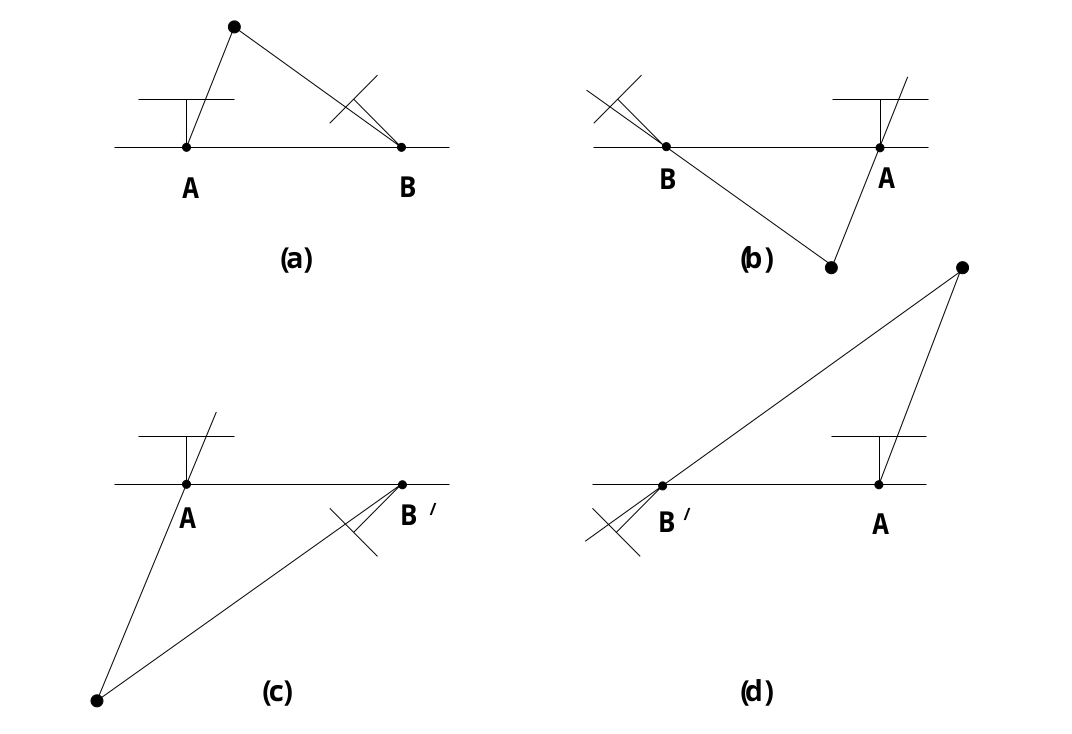
\includegraphics[width=10cm]{images/ep4sols.png}
	\caption[Four possible solutions retrieved from $E$]{Four possible solutions retrieved from the essential matrix $E$. The points A and B correspond to the centers of projection before and after rotating. Between the right side, (a) and (c), and the left side, (b) and (d), figures, there is a translation direction inversion. Between top, (a) and (b), and bottom, (c) and (d), figures, there is a rotation of 180 degrees around the baseline. \cite{multiview}}
	\label{sec2:fig:ep4}
\end{figure}

\subsection{Pure rotation}
\label{urerrrrr}
As a disadvantage of epipolar geometry, if the eye's movement is not constrained by a translation component, the epipolar relation will not work, since $[\mathbf{t}]_\times$ would be a $3x3$ matrix of zeros and, consequently, $E = [\mathbf{t}]_\times R$ would yield the same, making it impossible to retrieve the rotation.\\

When doing feature detection and matching, wrongly matched pairs of points between the two images, or points with large location errors, could severely affect the precision of the estimation of $F$. The reason for this is that all methods are least-square techniques that assume the noise which corrupts the data has zero mean. Hence, it is relevant to look into techniques of robust estimation.


%!TEX root = ../dissertation.tex

\section{Robust Estimation and Rejection of Image Sections}
\label{cha2:robustest}
